% !TeX root = ../../../book.tex
\section{定义与示例}

你通常是如何看待一个函数的?对函数的直观理解是什么?你会如何用数学对象来\emph{定义}函数呢?你以前尝试过这样定义函数吗?试试看吧!想想我们已经学过的概念和工具,能不能仅用这些概念来表达你对\emph{函数}的理解呢?认真试一下!先阅读接下来的几段内容,我们会逐步建立函数的定义,然后你再尝试自己给出一个定义。

我们通常认为函数是一种\emph{规则}或\emph{映射},用来告诉我们如何将输出值分配给任意给定的输入值。例如,定义在 $\mathbb{R}$ 上的函数 $f(x) = x^2$,它接受一个实数作为输入并输出该实数的平方。函数 $f$ 就像一台``机器'',把一个数字变成它的平方;说函数``在 $\mathbb{R}$ 上''意味着我们只能把实数放进这台机器。那么,我们怎么知道机器允许输出什么呢?我们已经发现了对函数解释中的一个缺陷。理想情况下,我们希望在定义函数时传达所有必要的信息:输入可以是什么,输出可以是什么(不一定是所有可能的输出,也可以是什么类型的对象),以及``规则''是什么。如果你把函数看作一个\emph{映射},那么它就像是描述如何通过某种集合间的``道路''(在这个例子中是取输入数的平方),从一组数字(在这种情况下是 $\mathbb{R}$)导航到另一组数字(也是 $\mathbb{R}$)。在这种解释中,我们仍然希望传达刚才提到的所有信息,但也指出了其他的理解方式。

在我们给出定义之前,先来思考一个问题。假设有一个``规则'',它的输入是一个人,而输出是这个人的眼睛颜色。你会如何将其表示为 $f(x) = \dots$ 的形式呢?这很难!你几乎需要将前一句话完整地重写,才能定义这个``规则''。那么,允许的输入和输出是什么呢?它们既不是实数也不是整数,而是完全不同的东西。然而,这个函数是合理的,我们希望在定义中包含它。思考一下这种情况与 $f(x) = x^2$ 在实数集 $\mathbb{R}$ 上的函数有何不同(或者实际上并没有什么不同)。(你甚至可能会反对说这根本就不是一个\emph{函数}!万一一个人有两种不同颜色的眼睛呢?这个``映射''的输出又是什么呢?哦,天哪!)

好了,现在轮到你了。试着用我们在前几章讨论过的概念、术语和数学对象来定义\emph{函数}。

% !TeX root = ../../../book.tex

\subsection{定义}

我们将使用以下定义。或许它与你的定义接近,甚至相同,或者只是措辞略有不同。但这个定义完美地概括了我们前面对函数的直观概念(将函数看作一种分配\emph{规则}),并用我们一直以来在发展的集合和逻辑语言来表达。这样做有几个好处:

\begin{enumerate}[label=(\alph*)]
    \item 它为函数提供了严格的基础,使我们能够在数学意义上放心地使用它们;
    \item 它让我们能够讨论函数的性质,并用数学术语和概念来证明这些性质;
    \item 它使我们能够概括函数的概念,并将其应用于比我们熟悉的标准数集更抽象的场景中。
\end{enumerate}
好了,解释到此为止,我们来看定义。\\

\begin{definition}
    设 $A, B$ 为集合。设 $f$ 为 $A, B$ 间的关系,所以 $f \subseteq A \times B$。同时假设 $f$ 具有如下性质:
    \[\forall a \in A \centerdot \exists! b \in B \centerdot (a, b) \in f\]
    (回想一下,``$\exists!$'' 表示``存在唯一的……'',也就是说``有且只有一个……'')

    这样的关系称为 $A$ 到 $B$ 的 \dotuline{函数}。

    我们称 $A$ 为函数的\dotuline{定义域},$B$ 为函数的\dotuline{值域}。

    写做
    \[f:A \to B\]
    表示 $f$ 是 $A$ 到 $B$ 的函数。

    如果 $(a,b) \in f$,则我们写做
    \[f(a) = b\]
    并且知道对于给定的 $a$,$b$ 是唯一满足该属性的元素。
\end{definition}

就是这样!虽然现在把\emph{函数}看作一种\emph{关系} --- 实际上是一种特殊的\emph{集合} --- 可能有点奇怪,但这正是它的本质。用这种方式定义函数让我们能够用集合和关系的语言来讨论它们,同时我们仍然可以使用一些熟悉的符号。对于每一个``输入'' $a$(即\emph{定义域}中的每一个元素),都有\emph{唯一}一个``输出'' $b$(即\emph{值域}中的一个元素)。因此,我们可以写成 $f(a) = b$,并且知道 ``$=$'' 表示真正的相等关系,因为只有这个唯一的 $b$ 满足这种关系。

这种定义的一部分包含了我们之前提到的想法:我们想知道函数会``输出''什么\emph{类型}的对象。这就是通过指定值域实现的。例如,定义函数 $f : \mathbb{R} \to \mathbb{R}$ 为 $f(x) = \sqrt{x}$ 是不合适的,因为定义域中的某些元素(即负数)会使``输出''未定义。(技术上讲,输出会是一个复数,而复数不是值域 $\mathbb{R}$ 的元素;在 $\mathbb{R}$ 的上下文中,我们认为复数是``未定义''的。)当一个函数被正确定义,且定义域和值域已明确,并且相关的对确实属于集合的笛卡尔积时,我们称这个函数是\textbf{良好定义的}。有时,我们会给出两个集合之间的关系,并要求你判断它是否是\emph{良好定义的函数}。实际上,这就是在问这个关系是否符合函数的定义。

\subsubsection*{范围}

\emph{值域}这个词对你来说可能比较陌生。实际上,你可能更习惯用\textbf{范围}来指代函数的\emph{潜在}``输出''集合。我们想在这个上下文中完全避免使用``范围''一词,因为它可能会产生歧义。有些作者和老师用``范围''来表示我们这里所说的``值域'',即函数的\emph{潜在}``输出''集合;而另一些人则用它来表示本书所说的``像'',即函数的\emph{实际}``输出''集合。在 \ref{sec:section7.3} 节中我们会详细定义这个术语。通常,像是值域的子集,但往往可能是\emph{真}子集。当有人使用``范围''这个词时,他们可能指的是这两种解释中的其中一个,而你可能理解的是另一个!为了避免这种混淆,我们将只使用\emph{值域}和\emph{像}这两个词。

% !TeX root = ../../../book.tex

\subsection{示例}

让我们使用新定义来考察几个函数及非函数的例子。在分析这些例子时,我们将介绍函数的正确定义与表示方法,并描述如何通过``可视化''更好地理解某些函数。

\subsubsection*{表示法}

定义函数有多种正确方式。以下是定义``实数平方函数''的三种正确方法:
\begin{quotation}
    定义函数 $f \subseteq \mathbb{R} \times \mathbb{R}$ 为 $(x, y) \in f \iff y = x^2$。

    定义函数 $f : \mathbb{R} \to \mathbb{R}$ 为 $f=\big\{(x,x^2) \mid x \in \mathbb{R}\big\}$。

    定义函数 $f : \mathbb{R} \to \mathbb{R}$ 为 $\forall x \in \mathbb{R} \centerdot f(x) = x^2$。
\end{quotation}

思考以上每种定义如何符合前文给出的函数定义。
\begin{itemize}
    \item 第一种直接表明函数是 $\mathbb{R}$ 到 $\mathbb{R}$ 的\emph{关系},其本质是有序对的集合;
    \item 第二种通过集合构建符表示 $f$,避免使用\emph{当且仅当}语句;
    \item 第三种则强调每个输入 $x \in \mathbb{R}$ 都有\emph{唯一}一个``输出''。
\end{itemize}

我们\emph{通常}采用第三种表示法,因为它更容易理解且符合我们对函数的直观认识。特殊情况下也会选用其他表示法——例如需要强调函数底层结构或简化书写时。但定义函数时务必明确四个关键要素:\emph{定义域}、\emph{值域}、\emph{函数名}及\emph{映射规则}或\emph{集合}。

如果你还是不太理解为什么在定义函数时指定\emph{值域}如此重要,可以从计算机编程角度来思考。定义函数时通常需要\emph{声明}输出变量的数据类型(具体取决于编程语言)。以 \verb|Java| 为例:
\begin{verbatim}
    public int PlusOne (int x) {
        return x+1;
    }
\end{verbatim}
上面代码定义了一个函数 (\verb|PlusOne|),输入一个整数 (\verb|x|),加一后输出另一个整数。其中 \verb|x| 前的 \verb|int| 是输入的数据类型(整型),函数名 \verb|PlusOne| 前的 \verb|int| 是输出的数据类型(整型)。\\

\begin{example}
    考虑一个将自然数转换为其二进制表示的函数,记为 $B$。根据定义,$B(1) = 1, B(2) = 10, B(10) = 1010$。该函数的定义域是什么?值域是什么?能否严格写出其定义\emph{规则},还是用文字描述更为适宜?

    我们可以这样定义此函数:设 $S$ 为所有由 $0$ 和 $1$ 构成的有限二进制字符串的集合,进而定义函数 $B : \mathbb{N} \to S$ 为
    \[B = \{(n, s) \mid n \in \mathbb{N} \;\text{且}\; s \;\text{为}\; n \;\text{的二进制表示}\}\]
\end{example}

\begin{example}
    再次考察``平方函数'':设 $f : \mathbb{R} \to \mathbb{R}$ 定义为 $\forall x \in \mathbb{R}, f(x) = x^2$。此函数与下列函数是否相同?
    \begin{itemize}
        \item 设函数 $g : \mathbb{R} \to \mathbb{C}$ 定义为
            \[\forall x \in \mathbb{R} \centerdot g(x) = x^2\]
        \item 设函数 $h : \mathbb{Z} \to \mathbb{R}$ 定义为
            \[\forall x \in \mathbb{Z} \centerdot h(x) = x^2\]
    \end{itemize}

    函数 $g$ 的值域虽为复数集,但实际上 $\mathbb{R} \subseteq \mathbb{C}$,因此所有有序对 $(x, x^2) \in g$ 仍然满足 $x \in \mathbb{R}$ 且 $x^2 \in \mathbb{R}$。从这个角度看,$f$ 和 $g$ 可视作\emph{同一}函数,可记作 $f = g$。稍后,我们将详细探讨两个函数相等的确切含义。目前,只需说明 $f$ 和 $g$ 对应的底层关系具有相同的实数有序对即可。理论上,函数 $g$ \emph{允许}输出值为复数,但由于定义域和``规则''的设定,这实际上不会发生。

    函数 $h$ 的定义域 $\mathbb{Z} \subset \mathbb{R}$(是 $\mathbb{R}$ 的真子集)。因此,函数 $f$ 中的有许多有序对并不属于函数 $h$。例如,$(\frac{1}{2}, \frac{1}{4}) \in f$ 但 $(\frac{1}{2}, \frac{1}{4}) \notin h$。换句话说,$f(\frac{1}{2}) = \frac{1}{4}$,但 $h(\frac{1}{2})$ 未\emph{良好定义},因为 $\frac{1}{2}$ 不属于 $h$ 的定义域。
\end{example}

\begin{example}
    函数也可以\textbf{分段}定义。例如,考虑定义在 $\mathbb{R}$ 上的\emph{绝对值函数}:

    设函数 $a : \mathbb{R} \to \mathbb{R}$ 定义为
    \[\forall x \in \mathbb{R} \centerdot a(x) = 
    \begin{cases}
         x &\text{如果\ } x \ge 0 \\
        -x &\text{如果\ } x < 0
    \end{cases}\]

    定义域中的每个元素都\emph{恰好}落入某一种情况,因此没有歧义。
\end{example}

\subsubsection*{``良好定义''的函数}

给定定义域、值域和对应``规则''或集合,如何判定其是否构成函数?以下定义提供了明确的判断标准:

\begin{definition}\label{def:definition7.2.5}
    给定定义域 $A$、值域 $B$ 和``规则''$f$,称 $f$ 是\dotuline{良好定义的函数},当且仅当
    \begin{enumerate}[label=(\arabic*)]
        \item 规则对 $A$ 的所有元素均有定义;
        \item 对于任意 $a \in A$,规则都输出集合 $B$ 中的唯一一个元素。
    \end{enumerate}
\end{definition}

让我们用一个例子来阐释此概念。后面我们还会看到一些非函数的例子,并且会再次引用\textbf{良好定义的函数}的定义。\\

\begin{example}
    设函数 $a : \mathbb{Z} \to \mathbb{N}$ 定义为
    \[\forall z \in \mathbb{Z} \centerdot f(z) = |2z + 1|\]
    我们怎么确定对于任意\emph{整数} $z$,$|2z + 1|$ 均为\emph{自然数}?这并不显而易见,需要进行证明。

    假设 $z \in \mathbb{Z}$ 满足 $z \ge 1$。则 $2z+1 \in \mathbb{Z}$ 且 $|2z+1| = 2z+1 \ge 3$。因此 $f(x) \in \mathbb{N}$。

    假设 $z \in \mathbb{Z}$ 满足 $z \le -1$。则 $2z+1 \in \mathbb{Z}$ 且 $2z+1 \le -1$。故 $f(x) = |2z + 1| \ge 1 \in \mathbb{N}$。因此 $f(x) \in \mathbb{N}$。

    假设 $z = 0$。则 $f(z) = |2 \cdot 0 + 1| = 1$,因此 $f(z) \in \mathbb{N}$。

    无论哪种情况,我们发现定义函数 $f$ 的``规则''确实会生成一个自然数,该数是\emph{值域}中的元素。且只生成唯一一个数。因此,这是一个良好定义的函数。
\end{example}

\begin{example}
    设 $P$ 为世上所有人的集合。函数 $b : P \to \mathbb{N} \cup \{0\}$ 定义为
    \[b = \{(p, n) \mid p \in P \land p \text{\ 有\ } n \text{\ 个姐妹}\}\]
    (请注意,为了练习,我们这里使用了一种强调集合的符号风格。此外,将数学符号和文字杂糅在一起可能看起来有些奇怪,例如 ``$b(p) = p \text{\ 有多少个姐妹}$''。)

    这是一个良好定义的函数吗?我们认为是的。假如你走到某人面前(即某个元素 $p \in P$),问他有多少个姐妹(即 $b(p)$ 的值)。他会告诉你一个非负整数,并且他们不可能给出两个\emph{不同的}数字。

    你可能会指出,在今天这个离婚和再婚普遍的社会中,很多人有\emph{同父异母或同母异父的姐妹} (half-sisters),而 $\frac{1}{2} \notin \mathbb{N} \cup \{0\}$。这个观点有其道理。但是,在``简化假设''下,假设每个人都有\emph{整数数量}的姐妹,这个函数是良好定义的。
\end{example}

\subsubsection*{恒等函数}

设 $S$ 为任意集合。是否\emph{必然}存在一个从 $S$ 到 $S$ 的函数?我们可以想到许多从 $\mathbb{R}$ 到 $\mathbb{R}$ 的函数,但如果 $S$ 是任意集合呢?能否保证存在从 $S$ 到 $S$ 的函数?答案是肯定的!回想讨论关系时曾考虑的类似问题(参见示例 \ref{ex:example6.2.9})。我们知道在集合 $S$ 上总能定义\emph{等价关系}:例如通过 $(x, y) \in R \iff x = y$ 定义 $R$。该关系由所有形如 $(x, x)$ 的有序对组成,其中 $x \in S$。这个关系是否构成函数?只需验证定义性质:每个输入是否对应唯一输出?确实如此!集合中任意元素仅等于其自身。因此 $R$ 确实是一个函数,我们称之为恒等函数。

\begin{definition}[恒等函数]
    设 $S$ 为集合。$S$ 上的\dotuline{恒等函数} $Id : S \to S$ 定义为
    \[\forall x \in S \centerdot Id(x) = x\]
\end{definition}

也就是说,恒等函数的``输出与输入完全相同''。(可以将其想象为一部懒惰的机器,仅原样输出输入内容。)

当涉及\emph{不同}集合的恒等函数时,为避免混淆,使用 $Id_S$ 表示``\textbf{集合 $S$ 上的}恒等函数''。

\subsubsection*{非函数示例}

有时候,在解决问题时,我们可能会提出集合间的``规则''并质疑其是否为函数。那么规则何时不构成函数?回顾\textbf{良好定义的函数}的定义(见定义 \ref{def:definition7.2.5}),可能失败的情形有三种:

\begin{itemize}
    \item 可能存在某个定义域中的元素\textbf{没有对应的``输出''}。
    \item 可能存在某个定义域中的元素\textbf{有多个``输出''}。
    \item 可能存在某个定义域中的元素只有一个``输出'',但该``输出''\textbf{不在值域中}。
\end{itemize}
以下示例说明了这些情况。\\

\begin{example}
    设函数 $G : \mathbb{N} \times \mathbb{N} \to \mathbb{N}$ 定义为
    \[\forall (a, b) \in \mathbb{N} \times \mathbb{N} \centerdot G(a, b) = a - b\]

    这\textbf{不是}一个良好定义的函数,因为定义域中的多个元素其输出不在值域中。例如,$(5, 10) \in \mathbb{N} \times \mathbb{N}$,此时 $G(5, 10) = -5$,但 $-5 \notin \mathbb{N}$。
\end{example}

\clearpage

\begin{example}
    设 $W$ 为所有英语单词的集合。定义 $A: W \to W$ 为输入单词,输出原单词的异序词(即字母相同但顺序不同的单词)。
    
    这\textbf{不是}一个良好定义的函数。例如,HI 和 FUNCTION 不存在异序词。而像 INTEGRAL 这样的单词存在多个(即非唯一)异序词:TRIANGLE, ALERTING, ALTERING……
\end{example}

% !TeX root = ../../../book.tex

\subsection{函数相等}

有时,两个函数虽然由不同的规则或公式定义,但实际上表示了相同的对应关系!此时,这两个函数\textbf{相等}。我们将先从函数符号的角度描述这一情形,再通过对应关系和集合符号加以证明。

两个函数\emph{相等}的条件是什么?首先,其定义域必须相同。若定义域不同,则其中一个定义域包含另一个定义域中不存在的元素。(例如,一个函数在某元素上有定义而另一个函数无定义,二者显然不等)。设集合 $A$ 和 $B$,以及函数 $f : A \to B$ 和 $g : A \to B$。$f$ 与 $g$ 相等需满足何种条件?函数的核心特征在于:对任意输入 $x \in A$,$f$ 和 $g$ 均有\emph{唯一}输出 $f(x)$ 和 $g(x)$。若 $f$ 与 $g$ 为同一函数,则必有 $f(x) = g(x)$!由此可得如下定理。

\begin{theorem}
   设 $A, B$ 为集合。并设 $f : A \to B$ 和 $g : A \to B$ 为函数。若
   \[\forall x \in A \centerdot f(x) = g(x)\]
   则称 $f$ 与 $g$ 相等,记作 $f = g$。
\end{theorem}

这确实是一个\emph{定理}。该思想虽直观,却并未在函数的\emph{定义}中明示,因此需要证明。为此,考察 $f$ 和 $g$ 的所有有序对。通过证明这些有序对相同,可以在集合意义上得出 $f = g$。以下采用\emph{双向包含}论证。

\begin{proof}
   设 $A, B$ 为集合,$f : A \to B$ 和 $g : A \to B$ 为函数,且满足 $\forall x \in A \centerdot f(x) = g(x)$。
   \begin{itemize}
      \item 首先,证明 $f \subseteq g$。\\
            给定 $(a,b) \in f$。因为 $f$ 为函数,这意味着 $f(a) = b$。由题设 $f(a) = g(a)$ 可得 $g(a) = b$。因此 $(a,b) \in g$。这表明
            \[(a, b) \in f \implies (a, b) \in g\]
            即 $f \subseteq g$。
      \item 接着,证明 $g \subseteq f$。\\
            给定 $(c,d) \in g$。因为 $g$ 为函数,这意味着 $g(c) = d$。由题设 $f(c) = g(c)$ 可得 $f(c) = d$。因此 $(c,d) \in f$。这表明
            \[(c, d) \in g \implies (c, d) \in f\]
            即 $g \subseteq f$。
   \end{itemize}
    
   综上,由 $f \subseteq g$ 和 $g \subseteq f$,可得 $f = g$。
\end{proof}

这为我们提供了一种简便的方法来证明两个函数相等,而不需要深入探讨它们的底层关系或集合结构。我们只需要证明两个函数对于定义域中的每一个元素,其输出是相同的。接下来,我们通过几个例子来说明这一点。\\

\begin{example}
    设 $A = \{-1, 0, 1\}$。定义函数 $f_1 : A \to \mathbb{Z}$ 和 $f_2 : A \to \mathbb{Z}$ 为
    \[\forall x \in A \centerdot \big(f_1(x) = x\big) \land \big(f_2(x) = x^3\big)\]
    证明 $f_1 = f_2$。由于定义域只包含三个元素,我们可以逐一检验输出。
    \begin{align*}
        f_1(-1) = -1 &= (-1)^3 = f_2(-1)\\
        f_1(0) = 0 &= 0^3 = f_2(0)\\
        f_1(1) = 1 &= 1^3 = f_2(1)
    \end{align*}
    可见,对于每个合法输入(即 $\forall x \in A$)函数 $f_1$ 和 $f_2$ 均有相同的输出(即 $f_1(x) = f_2(x)$)。因此 $f_1 = f_2$。
\end{example}

\begin{example}
    设 $B = \{1, 2, 3\}$。定义函数 $g_1 : B \to \mathbb{Z}$ 和 $g_2 : B \to \mathbb{Z}$ 为
    \[\forall n \in B \centerdot \big(g_1(n) = n^3-n^2-6\big) \land \big(g_2(n) = 5n^2-11n\big)\]
    证明 $g_1 = g_2$。定义域还是只有三个元素,所以我们可以直接验证所有输出相等。
    \begin{align*}
        g_1(1) &= 1^3 - 1^2 - 6 = 1 - 1 - 6 = -6 \\
        g_2(1) &= 5 \cdot 1^2 - 11 \cdot 1 = 5 - 11 = -6 
   \end{align*}
   \begin{align*}
        g_1(2) &= 2^3 - 2^2 - 6 = 8 - 4 - 6 = -2 \\
        g_2(2) &= 5 \cdot 2^2 - 11 \cdot 2 = 20 - 22 = -2
   \end{align*}
   \begin{align*}
        g_1(3) &= 3^3 - 3^2 - 6 = 27 - 9 - 6 = 12 \\
        g_2(3) &= 5 \cdot 3^2 - 11 \cdot 3 = 45 - 33 = 12
    \end{align*}

    可见 $\forall n \in B \centerdot g_1(n) = g_2(n)$,因此 $g_1 = g_2$。
\end{example}

以上两个例子的定义域较小,可以逐一检查每个元素。然而,并非所有情况都如此简单。有时需要考虑定义域内任意元素(因为待证性质以``$\forall$''量词开头),并据此展开分析。实际上,针对此类情形存在一种巧妙的方法,接下来我们将演示其具体实现。

给定 $n \in B$。由于 $g_1(n)$ 和 $g_2(n)$ 都属于 $\mathbb{Z}$,考虑它们的差
\begin{align*}
    g_1(n) - g_2(n) &= (n^3 - n^2 - 6) - (5n^2 - 11n) \\
    &= n^3 - 6n^2 - 11n - 6 \\
    &= (n - 1)(n - 2)(n - 3)
\end{align*}

(注意:可以通过简单地展开这三项的乘积来验证最后的等式。)

由于 $n \in B$,因此 $n$ 只可能是 $1,2,3$。在每种情况下,$(n - 1), (n - 2), (n - 3)$ 其中一项必定为零。因此
\[g_1(n) - g_2(n) = (n - 1)(n - 2)(n - 3) = 0\]
由此可得 $g_1(n) = g_2(n)$。此式对任意 $n \in B$ 都成立,故得出结论 $g_1 = g_2$。

需要指出的是,此法比``逐项验证''更复杂。我们是怎么知道要做差的呢?我们又是如何知道它会以这样的形式因式分解的呢?这正是数学的魅力所在!或许是通过思考如何解决更一般的问题从而得到某种巧妙的方法,因为在此情形下,定义域太大,根本无法逐一验证。或许是识别出 $B = \{1, 2, 3\}$ 隐含的因式分解结构。只要仔细思考,便可领悟此例是如何巧妙构造出来的!$\smiley{}$

让我们来看一个更复杂的函数相等问题。下例涉及若干对你来说可能陌生的概念,后续也不会深入讨论,然而鉴于这个问题的趣味性与启发性,所以将其呈现在这里。\\

\begin{example}
    本例中,我们将定义两个函数,并说明它们为何相等。设每个函数的定义域和值域为 $\mathbb{R}^2$(实平面)。接下来,通过几何方式(即视觉上)定义两个函数 $F_1$ 和 $F_2$。定义 $F_1$ 输入平面上的一个点 $p$,并输出将 $p$ 绕原点逆时针旋转 $90 \degree$ 后再根据原点镜像得到的点。定义 $F_2$ 输入点 $p$,并输出将 $p$ 顺时针旋转 $90 \degree$ 后得到的点。为了更好地理解这两个函数的含义,请看下页中 $F_1$ 和 $F_2$ 的示意图。
    
    我们声称在函数意义上 $F_1 = F_2$。通过尝试几个例子,我们发现这可能是成立的,因为我们无法找到反例,甚至你可能已经``看出''为什么它成立。但这些都不是严格的证明,而只是一种直观的理解方法。为了严格证明这个事实,我们需要使用一些超出本课程范围的数学工具和方法。因此,我们只会概述证明过程,并将技术细节留给感兴趣的读者探索。

    \begin{multicols}{2}
        \begin{center}
            {\begin{tikzpicture}
                \draw[latex-latex] (-3,0) -- (3,0); 
                \draw[latex-latex] (0,-3) -- (0,3); 
                \draw (0,0) -- (1.5,1.5);
                \node at (1.5, 1.5)[circle,fill,inner sep=2pt]{};
                \draw[shift={(1.6, 1.5)}] node[right] {$p$};
                \draw (0,0) -- (-1.5,1.5);
                \node at (-1.5, 1.5)[circle,fill,inner sep=2pt]{};
                \draw[rotate=45] (0,0) rectangle (0.3,0.3);
                \draw (0,0) -- (1.5,-1.5);
                \node at (1.5, -1.5)[circle,fill,inner sep=2pt]{};
                \draw[shift={(1.6, -1.7)}] node[right] {$F_1(p)$};
                \draw[dashed,-latex] (1.5, 1.5) .. controls (0.5, 2.5) and (-0.5, 2.5) .. (-1.4, 1.6);
                \draw[shift={(-0.5, 2.5)}] node[left] {\small 旋转 $90 \degree$};
                \draw[dashed,-latex] (-1.5, 1.5) .. controls (-2, 0) and (-1.5, -2) .. (1.4, -1.6);
                \draw[shift={(-1.0, -0.3)}] node[right] {\small 相对};
                \draw[shift={(-1.0, -0.7)}] node[right] {\small 原点};
                \draw[shift={(-1.0, -1.1)}] node[right] {\small 镜像};
            \end{tikzpicture}}
        \end{center}

        \begin{center}
            {\begin{tikzpicture}
                \draw[latex-latex] (-3,0) -- (3,0); 
                \draw[latex-latex] (0,-3) -- (0,3); 
                \draw (0,0) -- (1.5,1.5);
                \node at (1.5, 1.5)[circle,fill,inner sep=2pt]{};
                \draw[shift={(1.6, 1.5)}] node[right] {$p$};
                \draw (0,0) -- (1.5,-1.5);
                \node at (1.5, -1.5)[circle,fill,inner sep=2pt]{};
                \draw[shift={(1.6, -1.7)}] node[right] {$F_2(p)$};
                \draw[rotate=-45] (0,0) rectangle (0.3,0.3);
                \draw[dashed,-latex] (1.5, 1.5) .. controls (2.5, 0.5) and (2.5, -0.5) .. (1.6, -1.4);
                \draw[shift={(0.5, 0.3)}] node[right] {\small 旋转 $90 \degree$};
            \end{tikzpicture}}
        \end{center}
    \end{multicols}

    主要思想是:我们可以用\emph{向量}表示平面上的点,用\emph{矩阵}表示函数,并通过矩阵乘法描述函数对点的作用。如果你对矩阵或向量不太熟悉,不用担心;你可以跳过这个例子,不会错过关键内容!不过,如果你想进一步了解,我们可以这样解释:矩阵是实数数组,而向量是单列矩阵。例如,实平面上的点 $(1, 1)$ 可表示为向量 $\begin{bmatrix}
        1 \\
        1
     \end{bmatrix}$。向量的\emph{旋转}可以通过\emph{旋转矩阵}实现(你可能在中级物理课程,如电磁学或力学中学过)。例如,逆时针旋转 $90 \degree$ 的矩阵表示为:
     \[\begin{bmatrix}
        0 & -1 \\
        1 & 0
     \end{bmatrix}\]
     将点 $(a, b)$ 逆时针旋转 $90 \degree$,等价于将对应向量与此矩阵相乘,遵循标准矩阵乘法规则(即行与列对应元素相乘并相加)。例如,旋转点 $(1, 1)$:
     \[\begin{bmatrix}
        0 & -1 \\
        1 & 0
     \end{bmatrix}\begin{bmatrix}
        1 \\
        1
     \end{bmatrix} = \begin{bmatrix}
        0+(-1) \\
        1+0
     \end{bmatrix}=\begin{bmatrix}
        -1 \\
        1
     \end{bmatrix}\]
     结果正如预期!请参阅上方图片了解旋转的实际效果。

     类似地,顺时针旋转 $90 \degree$ 的矩阵可以表示为:
     \[\begin{bmatrix}
        0 & 1 \\
        -1 & 0
     \end{bmatrix}\]

     (注意这些项的相似性,这是有原因的,建议通过搜索引擎探索细节。)

   以原点为中心的镜像也可用矩阵乘法表示,但更简单的理解是:将两个坐标取相反数。例如,镜像 $(-1, 1)$ 得到 $(1, -1)$。

   这使我们能完整描述 $F_1$ 和 $F_2$ 的动作。由于 $F_1$ 表示``逆时针旋转 $90 \degree$ 后取反坐标'',因此可以写作:
    \[F_1\Bigg(\begin{bmatrix}
        a \\
        b
     \end{bmatrix}\Bigg) = -\begin{bmatrix}
        0 & -1 \\
        1 & 0
     \end{bmatrix}\begin{bmatrix}
        a \\
        b
     \end{bmatrix}=\begin{bmatrix}
        b \\
        -a
     \end{bmatrix}\]
     (负号用于取反操作)。由于 $F_2$ 表示``顺时针旋转 $90 \degree$'',可以写作:
     \[F_2\Bigg(\begin{bmatrix}
        a \\
        b
     \end{bmatrix}\Bigg) = \begin{bmatrix}
        0 & 1 \\
        -1 & 0
     \end{bmatrix}\begin{bmatrix}
        a \\
        b
     \end{bmatrix}=\begin{bmatrix}
        b \\
        -a
     \end{bmatrix}\]
     根据矩阵与向量的乘法规则,我们可以轻易看出,对于任意 $a$ 和 $b$,这两个表达式相等。因此,假如你熟悉旋转矩阵,这就证明了 $F_1 = F_2$!
\end{example}

% !TeX root = ../../../book.tex

\subsection{示意图}

在我们深入讨论函数的抽象性质及其证明方法之前,我们先介绍一种有助于表示函数的方法。需要强调的是,这种方法在数学上并不\emph{严谨},在\emph{证明}中使用可能不是最佳选择。(例如,在评分的作业中,即使你有正确的想法,可能也不会得满分。)然而,这种方法确实能直观地展示函数的工作原理,并帮助你发现问题并进行更严格的证明。特别是,这种方法在构造函数性质的\emph{反例}时非常有用。

\textbf{示意图}的概念类似于我们用\emph{韦恩图}表示集合。集合是元素的集合,而不是纸上的阴影圆圈,但这些阴影圆圈及其重叠可以帮助我们理解和描述集合。同样,函数是两个集合之间具有特定属性的关系,而不是像这样:

\begin{center}
    {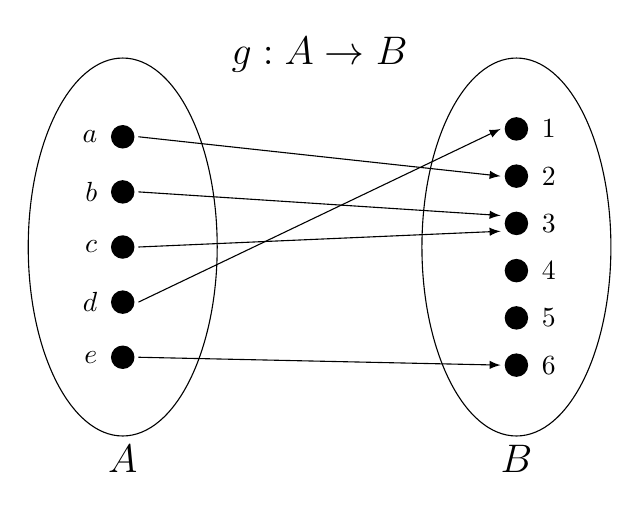
\begin{tikzpicture}[scale=1]
        \foreach \x in  {1,...,6}
        {
            \node at (5, -\x*0.6)[circle,fill,inner sep=3pt]{};
            \draw[shift={(5.2, -\x*0.6)}] node[right] {$\x$};
        }
        \draw (5,-2.1) ellipse (1.2 and 2.4);

        \foreach \x/\s in  {1/a,2/b,3/c,4/d,5/e}
        {
            \node at (0, -\x*0.7)[circle,fill,inner sep=3pt]{};
            \draw[shift={(-0.2, -\x*0.7)}] node[left] {$\s$};
        }
        \draw (0,-2.1) ellipse (1.2 and 2.4);

        \draw[-latex] (0.2,-0.7) -- (4.8,-1.2); 
        \draw[-latex] (0.2,-1.4) -- (4.8,-1.7); 
        \draw[-latex] (0.2,-2.1) -- (4.8,-1.9); 
        \draw[-latex] (0.2,-2.8) -- (4.8,-0.6); 
        \draw[-latex] (0.2,-3.5) -- (4.8,-3.6);
        
        \node[below] at (0, -4.5){\Large $A$};
        \node[below] at (5, -4.5){\Large $B$};
        \node[above] at (2.5, 0){\Large $g:A \to B$};
    \end{tikzpicture}}
\end{center}

然而,这在某种程度上确实\emph{代表}了函数的概念。在这幅图中,我们用椭圆分别表示了定义域 $A$ 和值域 $B$。$A$ 和 $B$ 的元素则用椭圆内的点来表示,并且进行了标记。我们根据函数 $g: A \to B$ 在这些点之间画上箭头。

这种方法通常用于探索函数的特性,或者构造反例来反驳某个主张。通过绘制一些点和箭头,并尝试它们的连接方式,我们可以逐步构建一个例子的基础\emph{结构}。然后,再为图中的各部分分配名称和公式,使其更加严谨。

在我们的讨论中,我们会用一些示意图来说明某些属性和概念,同时提供更严谨的陈述或描述。我们鼓励你也采用这种方法。

% !TeX root = ../../../book.tex

\subsection{习题}

\subsubsection*{温故知新}

以口头或书面的形式简要回答以下问题。这些问题全都基于你刚刚阅读的内容,如果忘记了具体定义、概念或示例,可以回顾相关内容。确保在继续学习之前能够自信地作答这些问题,这将有助于你的理解和记忆!

\begin{enumerate}[label=(\arabic*)]
    \item 在不查阅资料的情况下,写出\textbf{函数}的定义。然后,与我们的定义进行比较。你的定义是否传达了相同的信息?如果没有,遗漏了什么内容?
    \item 函数的\textbf{定义域}和\textbf{值域}有何区别?
    \item 函数\textbf{良好定义}的含义是什么?
    \item 什么是\textbf{恒等函数}?它是如何定义的?
    \item 如何证明两个函数\textbf{相等}?
\end{enumerate}

\subsubsection*{小试牛刀}

尝试解答以下问题。这些题目需动笔书写或口头阐述答案,旨在帮助你熟练运用新概念、定义及符号。题目难度适中,确保掌握它们将大有裨益!

\begin{enumerate}[label=(\arabic*)]
    \item 用符号定义函数:输入整数,输出其绝对值的平方根。\\
          该函数的定义域是什么?值域是什么?
    \item 用符号定义函数:输入一对自然数,输出其算术平均数。\\
          该函数的定义域是什么?值域是什么?
    \item 设 $A = \{-2, -1, 0, 1, 2\}$,定义 $g : A \to A$ 为 $\forall x \in A \centerdot g(x) = x^2 - 3$。绘制示意图来判断 $g$ 是否是良好定义的?
    \item 设 $X$ 为任意集合。用符号定义函数:输入 $X$ 的\emph{子集},输出其在 $X$ 上的补集。\\
          该函数的定义域是什么?值域是什么?
    \item 设 $B = \{-1, 0, 1\}$。定义 $h : B \to B$ 为 $\forall b \in B \centerdot h(b) = b^3$。这与哪个特殊函数相等?
    \item 设 $f : \mathbb{Z} \times \mathbb{Z} \to \mathbb{N}$ 为 $\forall (x, y) \in \mathbb{Z} \times \mathbb{Z} \centerdot f(x, y) = \frac{1}{2}|x + 1| \cdot |y|$。这是一个良好定义的函数吗?为什么?
\end{enumerate}